\section{Update phase}

  While the forward and backward pass perform cross--correlations and
  convolutions with a relatively large image with a small kernel
  producing another relatively large image, the cross--correlations
  performed during the update phase are performed on a large image
  with another large image resulting in a small image.

  Similarly as in the propagation algorithm, our update phase algorithm
  consists of the following stack of primitives.

  \begin{enumerate}
    \item {\bf Sub--kernel primitive} -- a primitive that computes a
      cross--correlation of each of $S$ images of size $R_Z \times R_Y
      \times (X + R_X - 1)$ with $S$ gradients of size $1 \times 1
      \times X$ to produce and accumulate the results of $S^2$ kernel
      gradients of size $R_Z \times R_X \times R_Y$.  As in the
      propagation algorithm, this primitive is optimized for efficiently
      reusing the register file as well as $L1$ cache.
    \item {\bf Full kernel primitive} -- a primitive that computes
      cross--correlation of an arbitrary sized $S$ images with
      arbitrary sized $S$ gradients to produce $S^2$ kernel gradients.
    \item {\bf Sub--layer primitive} -- a primitive that computes
      $\alpha \times \beta \times S^2$ kernel gradients by
      cross--correlating each of $\alpha S$ images with $\beta S$
      gradients.
    \item {\bf Full layer primitive} -- parallelized primitive that
      divides the computation into a set of previous primitives and
      statically schedules execution.  As described below, this
      primitive might need to contain an extra parallelized reduction
      step, which is also statically scheduled.
  \end{enumerate}


  \begin{algorithm}
    {\footnotesize
      \begin{codebox}
        \Procname{$\proc{Update-Subtask} \langle R_x, R_y, R_z, Z, R_s \rangle(i,\hat{i}',\Delta w)$}
        \li \kw{simd register} $oreg[R_x][R_y][R_z][R_s]$
        \li \kw{simd register} $wreg$
        \li \For $s_0 \gets 0 \To S/R_s - 1$
        \li \Do $oreg[:][:][:][s_0R_s:s_0R_s+R_s-1][:] \gets$
        \li   \Do $\proc{LOAD}(\Delta w[:][:][:][s_0R_s:s_0R_s+R_s-1][:])$
        \End
        \li \For $z_g \gets 0 \To Z-1$ \Comment Partially unrolled
        \li   \Do $wreg \gets \proc{LOAD}(\hat{i}'[1][1][z_g][:])$
        \li   \For $x \gets 0 \To R_x-1$ \Comment Fully unrolled
        \li   \Do \For $y \gets 0 \To R_y-1$  \Comment Fully unrolled
        \li   \Do \For $z \gets 0 \To R_z-1$  \Comment Fully unrolled
        \li   \Do \For $s_1 \gets 0 \To R_S-1$   \Comment Fully unrolled
        \li   \Do $oreg[x][y][z][s_0 \cdot R_s + s] \gets \proc{FMADD}($
        \li   \Do $wreg,$
        \li       $\proc{EXLOAD}(i[x][y][z+i][s_0 \cdot R_s + s]),$
        \li       $oreg[x][y][z][])$
        \End
        \End \li \kw{end for} $s$
        \End \li \kw{end for} $x$
        \End \li \kw{end for} $y$
        \End \li \kw{end for} $z$
        \End \li \kw{end for} $i$
        \li $\Delta w[:][:][:][s_0R_s:s_0R_s+R_s-1][:] \gets$
        \li \Do $\proc{STORE}(oreg[:][:][:][s_0R_s:s_0R_s+R_s-1][:])$
        \End
        \End \li \kw{end for} $s_0$
      \end{codebox}
    \caption{Serial update subtask.}
    \label{alg:serial-update-subtask}
    }
  \end{algorithm}

  {\bf Sub--kernel primitive} \quad The lowest level primitive is
  shown in Algorithm~\ref{alg:serial-update-subtask}.  Following the
  same principles as in the propagation sub--kernel primitive we
  vectorize the computation of $\Delta w[r_x][r_y][r_z][f][f']$ computed
  via {\small
  \[
  \sum_{z}
  a[r_x][r_y][r_z+z][f] \cdot b[r_x][r_y][r_z][f']
  \]
  } such that the values of $\Delta w[r_x][r_y][r_z][f][:]$ are computed
  via {\small
  \[
  \sum_{z}
  a[r_x][r_y][r_z+z][f] \cdot b[r_x][r_y][r_z][:]
  \]
  } Again, we recognize the reuse of $\hat{i}'[r_x][r_y][r_z][:]$ and
  re--order the loops appropriately.  In order to allow in--register
  computation, same constraints are imposed on $R_x \times R_y \times
  R_z \times R_s$ -- Maximal of $31$ for AVX512 and $8$ for SSE4, AVX
  and AVX2.  Additionally we allow only values for $R_s$ that divide
  $S$.  In order for the working set to fit inside the $L1$ cache, $Z$
  should be sufficiently small.  The number of bytes required for the
  working set equals $4S(R_xR_y+1)(R_z+Z-1)$.  For a given choice of
  $R_x, R_y$ and $R_z$, and given size of $L1$ cache, we
  conservatively choose $Z$ so that no more than half the cache is
  required for the working set.

   \begin{figure}
     \centering
     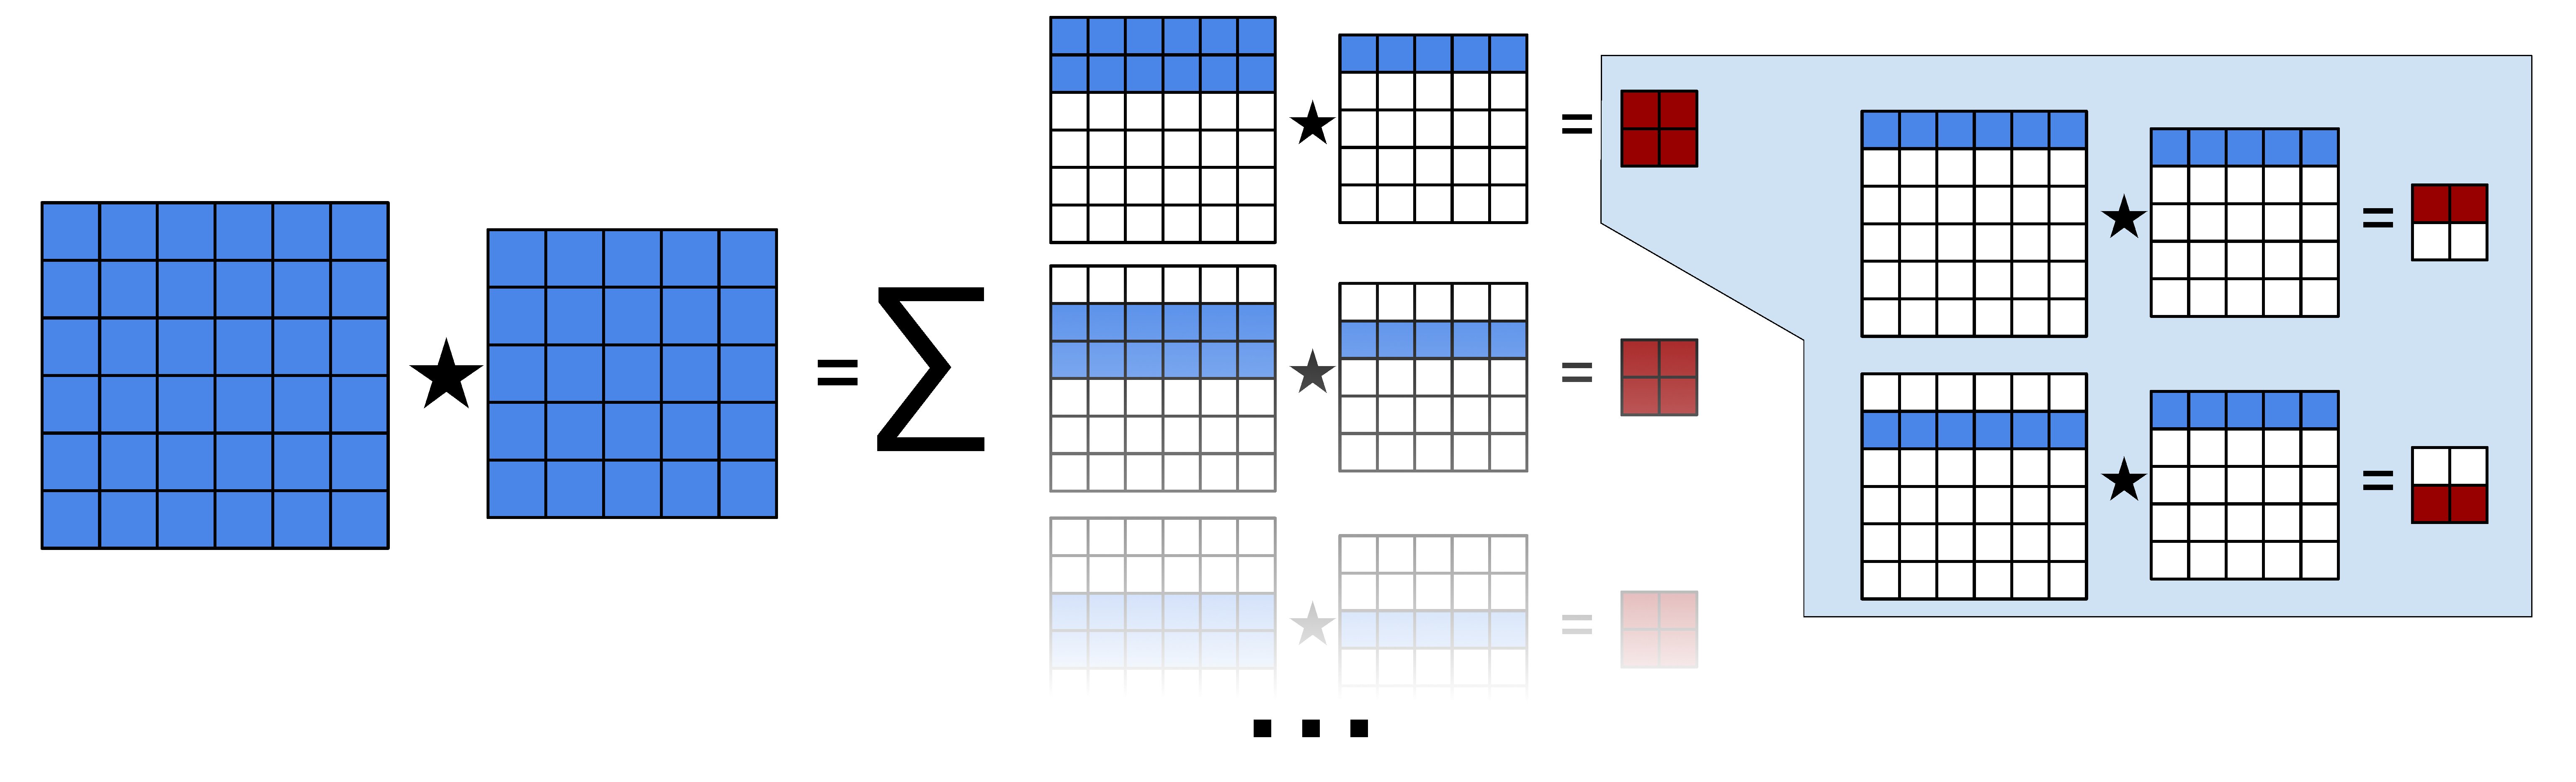
\includegraphics[width=0.99\linewidth]{fig/update2}
     \caption{An example of the {\bf full kernel primitive} and {\bf
         full gradient primitive} for the special case of $S=1$,...}
     \label{fig:conv-decomposition}
   \end{figure}

  {\bf Full kernel primitive} computes $S^2$ kernel gradients by
  cross--correlating each of $S$ images with $S$ gradients.  The
  computation is performed in two steps.  First, the gradients are
  split into sub--gradients of size $1 \times 1 \times Z$.  The result
  is then obtained as the sum of cross--correlations of each of the
  sub--gradients with an appropriate sub--image, as depicted on
  Fig~\ref{conv-decomposition} (middle column).  The
  cross--correlation of each sub--gradient is further split into
  sub--kernel primitives (right column on
  Fig.~\ref{conv-decomposition}.  We choose the $R_x, R_y, R_z$ and
  $R_s$ to maximize the register--file utilization, but subject to the
  limits described above.  Further, we require that $R_x, R_y$ and
  $R_z$ divide $K_x, K_y$ and $K_z$ respectively.  Note that this can
  always be accomplished be setting $R_x=R_y=R_z=1$ and $R_s=S$.
  However this choice might not be optimal.  For example, when $K_z=3$
  on AVX512 CPU, we could pick $R_s=8$ and $R_z=3$, which utilizes
  $24$ registers, which is better than choosing $R_z=1$ and
  $R_s=S=16$.  The optimal division is the one for which $R_x \times
  R_y \times R_z \times R_s$ is maximized.  When more combinations are
  possible, we prefer ones with large values of $R_s$, then $R_z$
  etc...  The value for $Z$ is then obtained using as described above.

  The computation is performed by iterating over the least significant
  dimension, then second least significant, etc..

  {\bf Sub--layer primitive} performs $\beta S \beta' S$
  cross--correlation.  Each of $\beta S$ input images is
  cross--correlated with each of $\beta'S$ output gradients to produce
  $\beta S \beta' S$ kernel gradients.  This primitive is designed for
  maximal reuse of higher levels of cache.  To achieve that, the
  computation is performed in the same fashion as in the propagation
  sub--layer primitive (Fig.~\ref{fig:full-exec}).

  {\bf Full layer primitive}, as in the propagation algorithm, divides
  the computation into sub--layer primitives which are scheduled for
  execution on $T$ threads.  In the propagation algorithm, all the
  divisions were done by splitting the large output tensor, allowing
  each thread to perform an independent computation.  As our update
  sub--layer primitive always computes full kernel gradients, the only
  sub--division into independently computer results is possible along
  the two most significant dimensions of $\Delta W$ tensor.

  Further division can be accomplished by dividing the computation
  over the input images and output gradients.  A division can be
  performed across the batches $B$, such that each thread considers
  only a subset of batches.  The resulting kernel gradients are then
  computed by accumulating the result obtained by each thread.
  Similarly, a division can be performed across the input image/output
  gradient as in the case of the {\bf full kernel primitive}.  This
  division also requires accumulating the results.

  To optimally divide the computation among threads we propose a two
  step scheduling algorithm.  In the first step, division along the
  two most significant dimensions of $\Delta W$ is performed to obtain
  independent sub--problems.  Let $P = \proc{GCD}(T,\alpha\alpha')$,
  we first select $\beta$ and $\beta'$ such that they divide $\alpha$
  and $\alpha'$ respectively, and $\beta\beta'P = T$.  Out of all
  possible values we pick the one for which $|\beta -\beta'|$ is
  minimized.  The threads are then also divided into $P$ sets of
  $T'=T/P$ threads, each of which will compute $\beta\beta'S^2$ kernel
  gradients.

  The values of the kernel gradient tensor $\Delta W(A
  \beta'S:A\beta'S+\beta'S-S,B \beta S: B\beta S + \beta S -S, :,:,:)$ is
  performed by the $A + B \alpha / \beta$-th set of $T'$ threads.

  In the second step, we divide the computation of each of
  $\beta\beta'S^2$ kernel gradients among the $T'$ threads in the set.
  When $T'$ equals $1$, the single thread in the set scheduled to
  perform the whole computation using a full layer primitive.

  When $T'>1$, we perform the division over input images and output
  gradients, creating a full layer primitive for each sub--problem.
  The division is performed in the same fashion as in the propagation
  algorithm, preferring division over $B$, then over $N_x'$, $N_y'$
  and finally $N_z'$.  However, each of the $T'$ threads in the set
  will accumulate the computed kernel gradients of each primitive into
  a local tensor.

  The $T'$ tensors computed by each thread have to be then accumulated
  to obtain the final kernel gradient tensor.  This is accomplished by
  performing a reduction step after all threads in the set have
  completed the execution. The reduction requires little computation
  compared to the overall computation performed by the layer, and is
  thus performed by a single thread in the set.
